%%%%%%%%%%%%%%%%%%%%%%%%%%%%%%%%%%%%%%%%%%%%%%%%%%%%%%%%%%%%%%%%%%%%%
%% This is a (brief) model paper using the achemso class
%% The document class accepts keyval options, which should include
%% the target journal and optionally the manuscript type.
%%%%%%%%%%%%%%%%%%%%%%%%%%%%%%%%%%%%%%%%%%%%%%%%%%%%%%%%%%%%%%%%%%%%%
\documentclass[journal=jacsat,manuscript=article]{achemso}

%%%%%%%%%%%%%%%%%%%%%%%%%%%%%%%%%%%%%%%%%%%%%%%%%%%%%%%%%%%%%%%%%%%%%
%% Place any additional packages needed here.  Only include packages
%% which are essential, to avoid problems later. Do NOT use any
%% packages which require e-TeX (for example etoolbox): the e-TeX
%% extensions are not currently available on the ACS conversion
%% servers.
%%%%%%%%%%%%%%%%%%%%%%%%%%%%%%%%%%%%%%%%%%%%%%%%%%%%%%%%%%%%%%%%%%%%%
\usepackage[version=3]{mhchem} % Formula subscripts using \ce{}
\usepackage[T1]{fontenc}       % Use modern font encodings

\usepackage{color}
\usepackage{xr}
\externaldocument{suppinfo}

%%%%%%%%%%%%%%%%%%%%%%%%%%%%%%%%%%%%%%%%%%%%%%%%%%%%%%%%%%%%%%%%%%%%%
%% If issues arise when submitting your manuscript, you may want to
%% un-comment the next line.  This provides information on the
%% version of every file you have used.
%%%%%%%%%%%%%%%%%%%%%%%%%%%%%%%%%%%%%%%%%%%%%%%%%%%%%%%%%%%%%%%%%%%%%
%%\listfiles

%%%%%%%%%%%%%%%%%%%%%%%%%%%%%%%%%%%%%%%%%%%%%%%%%%%%%%%%%%%%%%%%%%%%%
%% Place any additional macros here.  Please use \newcommand* where
%% possible, and avoid layout-changing macros (which are not used
%% when typesetting).
%%%%%%%%%%%%%%%%%%%%%%%%%%%%%%%%%%%%%%%%%%%%%%%%%%%%%%%%%%%%%%%%%%%%%
\newcommand*\mycommand[1]{\texttt{\emph{#1}}}

\newcommand{\cli}{Cl$^{-}$}
\newcommand{\ki}{K$^{+}$}

\newcommand{\tsveta}[1]{\textcolor{red}{#1}}
\newcommand{\denis}[1]{\textcolor{green}{#1}}

%%%%%%%%%%%%%%%%%%%%%%%%%%%%%%%%%%%%%%%%%%%%%%%%%%%%%%%%%%%%%%%%%%%%%
%% Meta-data block
%% ---------------
%% Each author should be given as a separate \author command.
%%
%% Corresponding authors should have an e-mail given after the author
%% name as an \email command. Phone and fax numbers can be given
%% using \phone and \fax, respectively; this information is optional.
%%
%% The affiliation of authors is given after the authors; each
%% \affiliation command applies to all preceding authors not already
%% assigned an affiliation.
%%
%% The affiliation takes an option argument for the short name.  This
%% will typically be something like "University of Somewhere".
%%
%% The \altaffiliation macro should be used for new address, etc.
%% On the other hand, \alsoaffiliation is used on a per author basis
%% when authors are associated with multiple institutions.
%%%%%%%%%%%%%%%%%%%%%%%%%%%%%%%%%%%%%%%%%%%%%%%%%%%%%%%%%%%%%%%%%%%%%
\author{Tsveta Miteva}
\affiliation{Sorbonne Universit\'{e}, CNRS, Laboratoire de Chimie Physique Mati\`{e}re et Rayonnement, UMR 7614, F-75005 Paris, France}
\email{tsveta.miteva@upmc.fr}


\author{Nikolai V. Kryzhevoi}
\affiliation{Theoretische Chemie, Physikalisch-Chemisches Institut, Universit\"at Heidelberg, Im Neuenheimer Feld 229, D-69120 Heidelberg, Germany}

\author{Nicolas Sisourat}
\affiliation{Sorbonne Universit\'{e}, CNRS, Laboratoire de Chimie Physique Mati\`{e}re et Rayonnement, UMR 7614, F-75005 Paris, France}

\author{Christophe Nicolas}
\affiliation{Synchrotron SOLEIL, l`Orme des Merisiers, Saint-Aubin, F-91192 Gif-sur-Yvette Cedex, France}

\author{Wandared Pokapanich}
\affiliation{Faculty of Science, Nakhon Phanom University, Nakhon Phanom 48000, Thailand}
%
\author{Thanit Saisopa}
\author{Prayoon Songsiriritthigul}
\affiliation{School of Physics, Suranaree University of Technology, Nakhon Ratchasima 30000, Thailand}
%
\author{Yuttakarn Rattanachai}
\affiliation{Department of Applied Physics, Faculty of Sciences and Liberal Arts, Rajamangala University of Technology Isan, Nakhon Ratchasima 30000, Thailand}

\author{Andreas Dreuw}
\author{Jan Wenzel}
\affiliation{Interdisciplinary Center for Scientific Computing, Ruprecht-Karls University, Im Neuenheimer Feld 205A, D-69120 Heidelberg, Germany}

\author{J\'{e}r\^ome Palaudoux}
\affiliation{Sorbonne Universit\'{e}, CNRS, Laboratoire de Chimie Physique Mati\`{e}re et Rayonnement, UMR 7614, F-75005 Paris, France}

\author{Gunnar \"{O}hrwall}
\affiliation{MAX IV Laboratory, Lund University, P.O. Box 118, SE-22100 Lund, Sweden}

\author{Ralph P\"{u}ttner}
\affiliation{Fachbereich Physik, Freie Universit\"at Berlin, Arnimallee 14, D-14195, Berlin, Germany}

\author{Lorenz S. Cederbaum}
\affiliation{Theoretische Chemie, Physikalisch-Chemisches Institut, Universit\"at Heidelberg, Im Neuenheimer Feld 229, D-69120 Heidelberg, Germany}

\author{Jean-Pascal Rueff}
\affiliation{Sorbonne Universit\'{e}, CNRS, Laboratoire de Chimie Physique Mati\`{e}re et Rayonnement, UMR 7614, F-75005 Paris, France}
\alsoaffiliation{Synchrotron SOLEIL, l`Orme des Merisiers, Saint-Aubin, F-91192 Gif-sur-Yvette Cedex, France}

\author{Denis C\'{e}olin}
\email{denis.ceolin@synchrotron-soleil.fr}
\affiliation{Synchrotron SOLEIL, l`Orme des Merisiers, Saint-Aubin, F-91192 Gif-sur-Yvette Cedex, France}

%%%%%%%%%%%%%%%%%%%%%%%%%%%%%%%%%%%%%%%%%%%%%%%%%%%%%%%%%%%%%%%%%%%%%
%% The document title should be given as usual. Some journals require
%% a running title from the author: this should be supplied as an
%% optional argument to \title.
%%%%%%%%%%%%%%%%%%%%%%%%%%%%%%%%%%%%%%%%%%%%%%%%%%%%%%%%%%%%%%%%%%%%%
\title{The all-seeing eye of resonant Auger electron spectroscopy: a study on aqueous KCl}

%%%%%%%%%%%%%%%%%%%%%%%%%%%%%%%%%%%%%%%%%%%%%%%%%%%%%%%%%%%%%%%%%%%%%
%% Some journals require a list of abbreviations or keywords to be
%% supplied. These should be set up here, and will be printed after
%% the title and author information, if needed.
%%%%%%%%%%%%%%%%%%%%%%%%%%%%%%%%%%%%%%%%%%%%%%%%%%%%%%%%%%%%%%%%%%%%%
\abbreviations{AES,XAS}
\keywords{Solvated ions, Auger spectroscopy, X-ray absorption spectroscopy}

%%%%%%%%%%%%%%%%%%%%%%%%%%%%%%%%%%%%%%%%%%%%%%%%%%%%%%%%%%%%%%%%%%%%%
%% The manuscript does not need to include \maketitle, which is
%% executed automatically.
%%%%%%%%%%%%%%%%%%%%%%%%%%%%%%%%%%%%%%%%%%%%%%%%%%%%%%%%%%%%%%%%%%%%%
\begin{document}


\begin{figure}[h!]
\centering
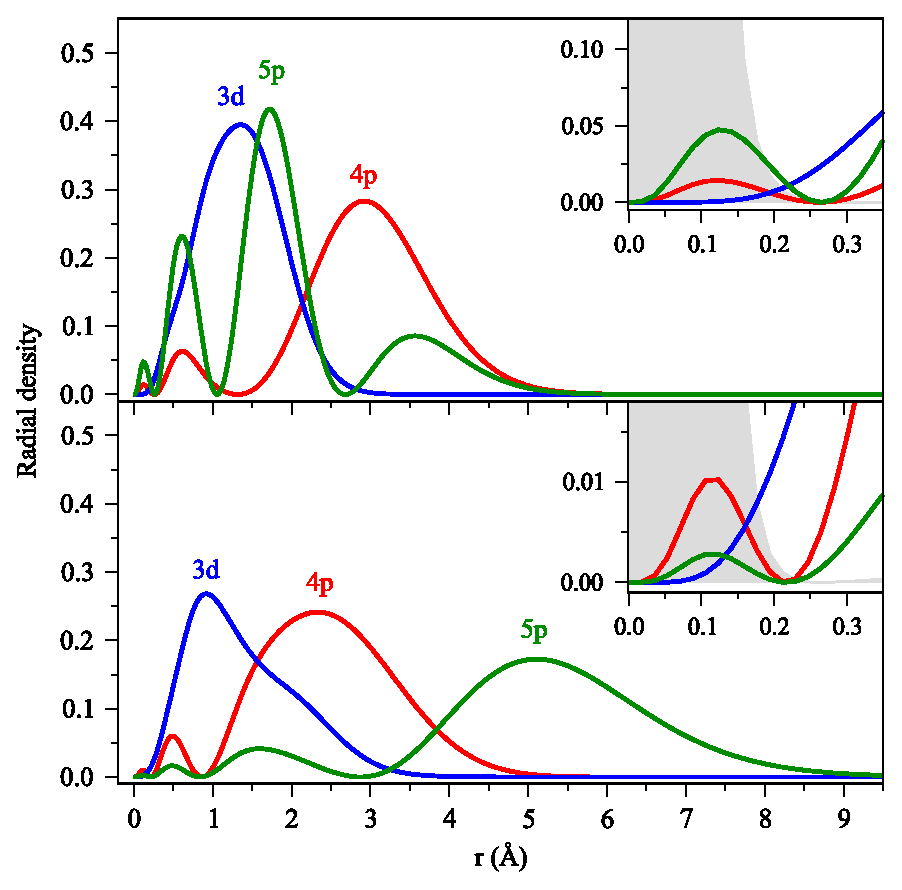
\includegraphics[scale=0.8]{figures/rad_dens_kcl.eps}
\caption{Radial density distributions of the singly-occupied natural orbital occupied by the excited electron corresponding to the 1s$^{-1}$4p, 1s$^{-1}$3d and 1s$^{-1}$5p core excitations in \ki~(lower panel) and \cli~(upper panel). The insets show the region of distances relevant for the overlap with the 1s core orbital whose radial density is shown as a grey shaded area.}
\label{fg:si_rdens_ions}
\end{figure}
{\color{red}
In what follows we give a tentative explanation of the difference in the radial density distributions of the 1s$^{-1}$4p and 1s$^{-1}$5p states in \ki~and \cli. In the case of \ki, the excited electron mainly sees a $2/r$ potential. In addition, it sees a short range potential coming from the pointlike nucleus and the screening electrons. The latter one normally leads to a quantum defect different from 0. Beside this one has Rydberg series with an infinite number of states. However, in case of Cl- the outer electron does not see a Coulomb potential and the short-range potential becomes dominant. As a result we see the unusual behaviour, like e.g. a finite number of bound states (here obviously 4p). In contrast to this 3d and 5p are in the continuum.}


\begin{figure}
\centering
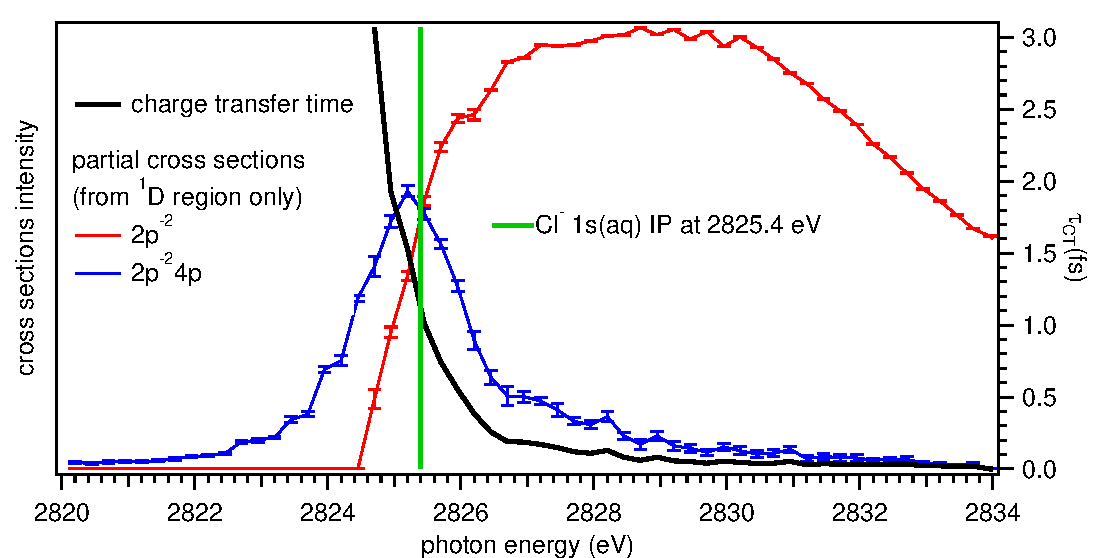
\includegraphics[scale=0.9]{figures/partial_cross_sec_ct_time.pdf}
\caption{Partial cross sections and charge transfer time extracted from Fig.\ \ref{fg:2dmap_cl}. The blue and red curves are obtained by integrating the area of the 2p$^{-2}$ and 2p$^{-2}$4p final states ($^1$D state region only) at each photon energy step. From these curves we determine the charge transfer time $\tau_{\text{CT}}$ according to the formula $\tau_{\text{CT}} = \tau l/d$, with $\tau$ being the Cl 1s core-hole lifetime and $l/d$ being the intensity ratio of the localized (2p$^{-2}$ 4p) and delocalized (2p$^{-2}$) states at a given excitation energy \cite{foehlisch05:373}.  The green line defines the Cl$^{-}_{\text{aq}}$(1s) ionization potential.}
\label{fg:si_ct_time}
\end{figure}


%%%%%%%%%%%%%%%%%%%%%%%%%%%%%%%%%%%%%%%%%%%%%%%%%%%%%%%%%%%%%%%%%%%%%
%% The appropriate \bibliography command should be placed here.
%% Notice that the class file automatically sets \bibliographystyle
%% and also names the section correctly.
%%%%%%%%%%%%%%%%%%%%%%%%%%%%%%%%%%%%%%%%%%%%%%%%%%%%%%%%%%%%%%%%%%%%%
\bibliography{F:/Articles/bibliography/Bibliography}
%\bibliography{Bibliography}

\end{document}
